\chapter{Research Context}
Highly automated driving is currently an immensely attractive field for both academic and industrial research groups. 
A fully autonomous vehicle, which is able to tackle challenging driving situations without external input comparable to a human driver's performance, is yet to be build.
In this thesis, we propose a novel approach to knowledge and information representation for automotive environment models using cognitive modelling techniques.
More precisely, we adopt \acfp{VSA}, which are commonly used in tasks like cognitive modelling and natural language processing, for the specific application of automotive environment modelling.
To our knowledge, \acp{VSA} have not been applied in this particular context. 
In order to put our work in context of the current research landscape and to circumscribe this thesis, we need to review related work from several different areas like automated driving and mobile robotics, computational neuroscience, artificial intelligence and neuromorphic engineering.
A comprehensive overview for all of these research areas is out of scope of a single thesis.
However, we aim to cover the most significant results from all areas at least briefly, whereas we present an in-depth review of relevant work related to the thesis at hand, where necessary.

\section{Automated Driving}
"Robotics is the science of building computer-controlled mechanical devises, which are able to perceive and manipulate the physical world" \cite{Thrun2005}.
Automated driving in automotive context is a special case of robotics, since an autonomous vehicle can be considered a wheeled mobile robot, which is able to fulfill the transportation capabilities of a traditional car without human input. 
In order to navigate safely to a desired goal, a mobile robot needs to solve several problems like localization ("where am I?"), path planning ("how do I get from A to B?"), environment perception ("where is everyone else?"), knowledge representation and reasoning ("which decisions to infer from available information?") as well as motion control ("how to move my actuators?").
In automotive context, an automated vehicle furthermore needs to detect the current state of the driver ("what is the driver up to") to ensure that he can take over control in safety-critical situations or in case of malfunctions.
The human driver as a fallback option in such situations is of crucial importance, since the level of driving automation gradually increases instead of a hard transition to automated driving systems.
In their J3016 standard \cite{SAE_J3016}, the \ac{SAE} delivers a classification system identifying six different levels of driving automation from "no automation" to "full automation".
Table \ref{tab:autonomy_levels} gives an overview of the particular automation levels according to \cite{SAE_J3016} in more detail.\\
On the road to fully automated driving, several \ac{ADAS} have been developed during the last decades and thus made a huge jump by incrementally increasing complexity and therefor the level of autonomy.
The history of automated driving research goes back to the 1980's, when governmental institutions funded several explorative projects worldwide to research functionalities like automatic vehicle driving and intelligent route planning resulting in early prototypes.
In 1986, several European research groups and vehicle manufacturers started the \ac{PROMETHEUS} project \cite{Dickmanns1990} and demonstrated a variety of different approaches to automated driving.
Another research initiative established during that period is Carnegie Mellon University's Navlab \cite{Thorpe1988}, which achieved the first completely autonomous drive from Pittsburg to San Diego.
After that first explorative phase, the US government established the \ac{NAHSC} in 1995 and shortly shortly followed by the foundation of the \ac{AHSRA} 1996 in Japan.
The main contribution of this first phase was the identification and deep analysis of problems, that would need to be tackled by researchers, to understand requirements and possible effects of future automated vehicles.
\cite{Bertozzi2000} gives an overview of the achievements and perspectives obtained in the projects during that period.\\
\begin{center}
	\begin{tabular}{|c | l | p{10cm}|}
		\hline
		\textbf{Level} & \textbf{Name} & \textbf{Narrative Definition}\\ \hline
		0 & No Automation & the full-time performance by the human driver of all aspects of the dynamic driving task, even when enhanced by warning or intervention systems \\ \hline
		1 & Driver Assistance & the driving mode-specific execution by a driver assistance system of either steering or acceleration/deceleration using information about the driving environment and with the expectation that the human driver perform all remaining aspects of the dynamic driving task \\ \hline
		2 & Partial Automation & the driving mode-specific execution by one or more driver assistance systems of both steering and acceleration/deceleration using information	 about the driving environment and with the expectation that the human driver perform all remaining aspects of the dynamic driving task \\ \hline
		3 & Conditional Automation &  the driving mode-specific performance by an automated driving system of all aspects of the dynamic driving task with the expectation that the human driver will respond appropriately to a request to intervene \\ \hline
		4 & High Automation & the driving mode-specific performance by an automated driving system of all aspects of the dynamic driving task, even if a human driver does not respond appropriately to a request to intervene \\ \hline
		5 & Full Automation & the full-time performance by an automated driving system of all aspects of the dynamic driving task under all roadway and environmental conditions that can be managed by a human driver \\ \hline
	\end{tabular}
	\label{tab:autonomy_levels}
	\captionof{table}{Table depicting different levels of vehicle automation identified in \cite{SAE_J3016}}
\end{center}
A major milestone in the research field of automated driving was the first \ac{DARPA} Grand Challenge in 2004, where unmanned vehicles had to complete a \SI{240}{\kilo\meter}, unrehearsed off-road course autonomously through the Mojave Desert in Nevada to win the price money of \$1 million. 
Although no participating vehicle successfully finished the race \cite{Bacha2004} in the first challenge, valuable insights have been gained.
Using those insights to make significant progress, five teams (out of 23) were able to successfully complete the second \ac{DARPA} Grand Challenge in 2005 with Stanford's Stanley robot winning first place \cite{Thrun2006}.
After the success of the second Grand Challenge, the \ac{DARPA} organized the Urban Challenge in 2007, switching the focus to automated driving in urban environments \cite{Buehler2009}.
In this competition, vehicles had to complete a \SI{97}{\kilo\meter} urban area course autonomously in less than \SI{6}{\hour}, while obeying California state driving laws, avoiding other participating vehicles and other objects using only on-board sensors and \ac{GPS}.
Six vehicles out of the 11 final participants successfully finished the competition, with Carnegie Mellon's Boss robot \cite{Urmson.2008} being named the winner finishing the course in little over \SI{4}{\hour} with an average speed of approximately \SI[per-mode=symbol]{22.5}{\kilo\meter\per\hour}.
\\
The technology developed for the \ac{DARPA} challenges formed the basis for commercial \ac{ADAS}, which have seen rapid progress since then and gradually made their way into series-production vehicles.
There exists a large variety of commercial systems, like e.g. \ac{ACC} or intelligent parking assistance systems, modern vehicles are already equipped with.
These systems have the potential to increase comfort and safety in road traffic and, in the long run enable fully autonomous driving (cf. Level 5 in Table \ref{tab:autonomy_levels}). 
On the other hand, many research teams and initiative were spawned or inspired from \ac{DARPA} Challenges these competitions and continued their research work after the .
\begin{figure}[t!]
	\centering
	\resizebox{.9\textwidth}{!}{%
	\subfloat[\label{subfig:stanley}]{%
		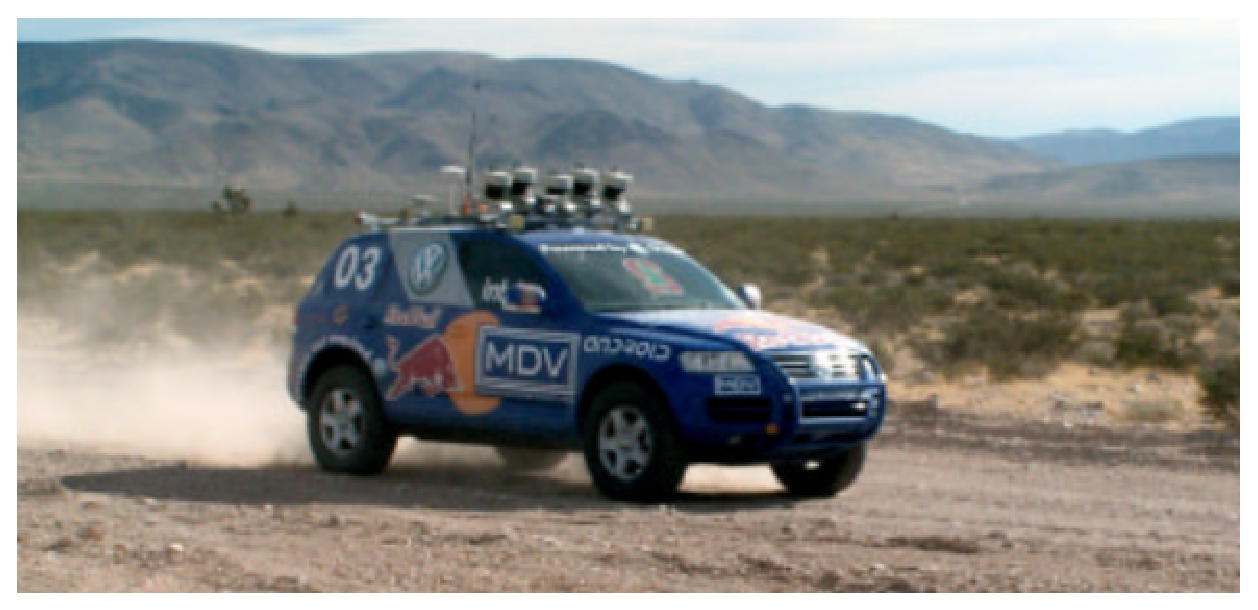
\includegraphics[height=3cm]{imgs/Stanley.eps}
	}
	\subfloat[\label{subfig:boss}]{%
		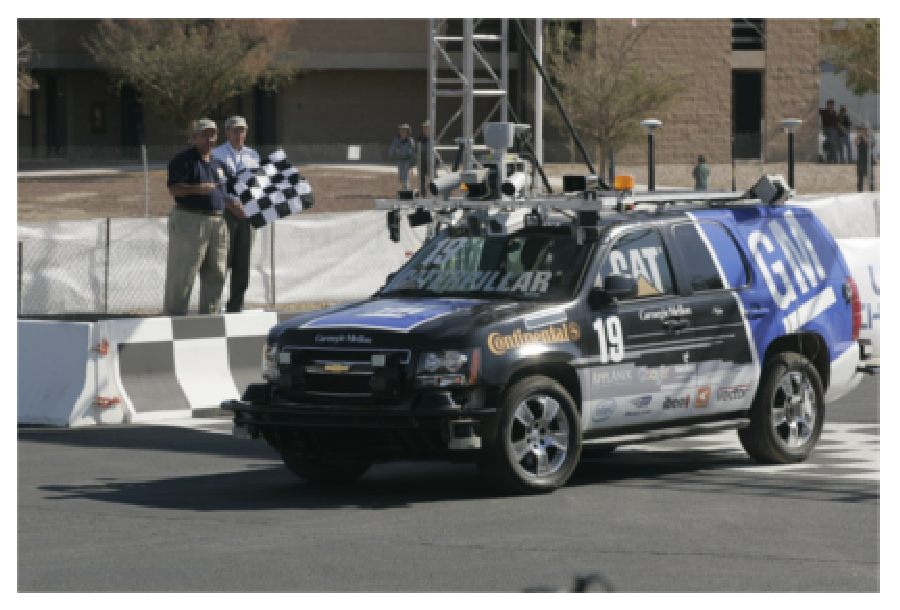
\includegraphics[height=3cm]{imgs/Boss_DARPA_urban_challenge.eps}
	}
}
	\caption{The winning robots from the 2005 \ac{DARPA} Grand Challenge and 2007 Urban Challenge. Fig. \ref{subfig:stanley} shows Stanford's Stanley at the 2005 \ac{DARPA} Grand Challenge (Image from \cite{Thrun2006}), Fig. \ref{subfig:boss} shows Carnegie Mellon's BOSS at the 2007 \ac{DARPA} Urban Challenge (Image from \cite{Urmson.2008}).}\label{fig:darpa_chal}
\end{figure}
Many researchers involved in the winning teams continued their research within Google's self-driving car project, which started in 2009 and evolved into the Spin-Off company Waymo \cite{Waymo} in 2016.
Another research team continuing their efforts after the \ac{DARPA} challenges is the Annieway team \cite{Annieway}.
One of their major contributions is the release and maintenance of the KITTI vision benchmark suite \cite{Geiger2013IJRR}, a publicly available data set containing data from various test drives in the city of Karlsruhe, rural areas as well as highways focusing on providing real world data for vision tasks like stereo, optical flow and 3D object detection and tracking.\\
The main research goal after the \ac{DARPA} Challenges was to develop automated driving with off-the-shelf sensors \cite{Furgale2013}.
As this thesis focuses on environmental modelling in context of autonomous driving, this section presents research from this field like road detection and modelling (Sec. \ref{subsec:lane}), object detection (Sec. \ref{subsec:obj_detect}) and tracking (Sec. \ref{subsec:obj_track}) as well as sensor fusion (Sec. \ref{subsec:sensor_fusion}) while other aspects like localization \cite{Levinson2010, Thrun2005}, path planning (\todo{citation}) and motion control (\todo{citation}) are neglected.
\subsection{Knowledge Representation}
\label{subsec:knowledge_representation}
\subsection{Object Detection and Classification}
\label{subsec:obj_detect}
\subsection{Behaviour Analysis}
\label{subsec:behav_analysis}
\section{Neuromorphic Systems}
To fully understand biological systems like the brain, which evolved over millions of years, is an ongoing yet unsolved challenge in biology and neuroscience.
Even small animals like insects or rodents show remarkable behavioural flexibility and the ability to constantly adapt to a rapidly changing and noisy world, which is unmatched by modern computing machines.
Mammals and primates are able to perform more sophisticated behaviours culminating in complex cognitive computations humans are capable of doing like thinking, problem solving, memory, reasoning, decision making, strategic planning, knowledge representation, learning etc.
The "biological computer" enabling these behaviours and cognitive abilities is the brain consisting of large networks of neural cells (or neurons), which communicate by sending and receiving electric signals via synapses.
At the same time, brains are comparably small and efficient: the human brain for example consumes only \SI{20}{\watt} of power (equivalent to a compact fluorescent light bulb) and comprises \SI{2}{\percent} of the body weight \cite[Chap. 2.1]{Eliasmith2013}. \\
Several research fields like computational neuroscience, neuromorphic engineering and neurorobotics try to reverse engineer biological systems to achieve similar performance and computational power.
During the last decades, researchers and engineers strived to close the gap in performance and efficiency between biological and artificial computing systems by mimicing neuro-biological architectures in hardware and implementing models of neural systems in software.
This biologically inspired, \textit{neuromorphic} approach promises not only to perform computations in a more efficient way, but also to tackle problems unsolvable with current computing machines.
\subsection{Historical remarks}
\begin{figure*}[t!]
	\centering
	\includegraphics[width=0.95\textwidth,height=270px, natwidth=944,natheight=350]{imgs/Neuromorphic_Timeline_alpha.png}
	\caption{Historical developments in computational neuroscience, neuromorphic engineering and machine learning.\todo{check and possibly update this figure}}
	\label{fig:neuro_time}
\end{figure*}

The term neuromorphic itself was first introduced by Carver Mead in the late 1980s \cite{Mead90}, when describing one of the first silicon retinas.
He called artificial systems that share organization principles with biological nervous systems neuromorphic.
An interesting prototype of a silicon retina, which is now considered a milestone, was implemented by Misha Mahowald, a PhD student of Carver Mead. 
Her thesis received Caltech's Milton and Francis Clauser Doctoral Prize for its originality and potential for opening up new avenues of human thought and endeavor.
Since these early days of neuromorphic engineering, the term has widely been used to describe \ac{VLSI} systems \cite{Mead1989}, novel computing devices \cite{Schemmel2010}, sensory systems \cite{Lichtsteiner2008, Liu2010}, software \cite{Davison2008, Bekolay2014} and algorithms \cite{ReverterValeiras2016}.
Considering the number of scientists, neuromorphic engineering is still a comparably young field of research but received an increased interest during the last decade from both academic and industrial research groups caused by the funding of large, ambitious projects.
Although there have been several achievements in the field during the 1990s \cite{Mead1989, Mahowald1992, Indiveri1997, Cauwenberghs1998} and early 2000s \cite{Liu2002}, the \ac{FACETS} project \cite{FACETS-proj} and the \ac{BBP} \cite{BlueBrain-proj}, both starting in 2005 and mainly funded by the \ac{EU} under the FP6-\ac{FET} program, were among the first big-budget neuromorphic projects.
The follow-up project \ac{BrainScaleS} \cite{BrainScaleS-proj, Schemmel2010} (2011-2015) built on and extended the research conducted during the \ac{FACETS} project. 
The main developments of the \ac{FACETS} and \ac{BrainScaleS} projects are the \ac{HICANN} chip \cite{Schemmel2010} and the Python-based simulator-independant language \ac{PyNN} \cite{Davison2008} for building neural network models.
Building on \ac{BBP} the \ac{BrainScaleS} hardware development is currently continued in the neuromorphic computing platform of \ac{HBP} \cite{HBP-proj, Calimera2013}, a large ten-year research project, which was selected as one of the two \ac{EU}-\ac{FET} flagships in 2013 and is granted around one billion euros funding.
Another project starting in 2005, initially funded by the UK government until 2014 and now also part of the neuromorphic computing platform of \ac{HBP}, is the \ac{SpiNNaker} project \cite{Furber2014} during which the neuromorphic computing hardware of the same name was developed.
The \ac{HBP} is organized in thirteen platforms in total, which focus on different research fields related to the brain like for example theoretical neuroscience, neurorobotics, cognitive architectures, high performance computing, brain simulation and the aforementioned neuromorphic computing platform (see \cite{HBP-proj} for details).\\
Beside these research activities in Europe, the \ac{DARPA} funded another big-budget neuromorphic project: the \ac{SyNAPSE} program \cite{SYNAPSE-proj, Srinivasa2012}, which started in 2008 and is scheduled to run until 2016, has received 102.6 million US dollars in funding as of January 2013. 
The program aims to build an electronic microprocessor system that matches a mammalian brain in function, size, and power consumption.
Achievements during the \ac{SyNAPSE} program, which is primarily contracted to IBM Research and \acs{HRL}, so far are include brain simulations, design of brain-inspired neuromorphic achitectures \cite{Nere2012} and the development of a digital neurosynaptic core \cite{Merolla2011}, which is a building block of IBM's recently published TrueNorth chip \cite{Akopyan2015}.
Further project results are the Corelet language \cite{Amir2013} and the simulator Compass \cite{Preissl2012}, which enable dedicated software development as well as simulation and testing of TrueNorth algorithms on standard hardware respectively.\\
Beside these projects, the neuromorphic community is coming together at two annual (three- resp. two-week) workshops in Telluride and CapoCaccia, which have been established in 1994 and 2007 respectively, to discuss the current state of research in lectures and interactive talk sessions, to forge new ideas and to work on hands-on projects in small workgroups.\\
The original definition of neuromorphic engineering also covers \acp{ANN} in general.
This research field even goes back to the 1940s when McCulloch and Pitts introduced artificial neurons as computational units \cite{McCulloch1988}, which embody a simplified model of biological neurons.
These first simple networks were able to calculate compositions of basic logic functions \cite{McCulloch1988, Rojas1996}.
Rosenblatt \cite{Rosenblatt58} proposed the first neural network, which was capable of learning, by adding numerical weights to the connections of the network with threshold functions as activation functions: the \textit{perceptron}.
Minsky and Papert \cite{Minsky1969} showed, that single-layer perceptrons are not able to calculate an XOR-function or, more generally, are only capable of learning linearly separable patterns.
This caused a decreased interest in neural networks research until the rediscovery of the backpropagation algorithm \cite{Werbos1974} in the 1980s \cite{Rumelhart1988}, which introduced a practically feasible method to optimize the network weights using gradient descent and led to a resurgence of neural network research.
%This gradient descent called for continuous activation functions (mostly sigmoid or hyperbolic) instead of threshold-functions as activation functions, which made the so-called second generation \ac{ANN} universal approximators for continuous functions \cite{Cybenko1989}.
Since then, various different network architectures like feed-forward, \acp{CNN}, \acp{RNN}, \acp{RBF}, \acp{RBM}, \acp{SOM} and \ac{ART} just to name a few \cite{Schmidhuber2015} have been proposed for different learning paradigms.
Although several simpler methods like Boosting \cite{Freund1997} or \acp{SVM} \cite{Vapnik1995} have been developed and achieved noteworthy results, the availability of powerful, parallelized computing hardware like \acp{GPU} as well as the advent and success  of deep learning (partly achieving better-than-human accuracy) made \acp{ANN} \cite{Rojas1996} and especially \acp{DNN} \cite{LeCun2015} the state-of-the-art for several machine learning tasks like visual digit \cite{Ciresan2012a} and traffic sign \cite{Ciresan2012} recognition in recent years.
Another great achievement in the field of deep learning was the victory of AlphaGo \cite{Silver2016} over the world's best Go player Lee Sedol in March 2016, which was considered to be at least a decade away due to the complexity of Go.
Compared to Deep Blue, the system that beat former chess world champion Garri Kasparov in 1997 \cite{Hsu2002} with sheer computational power by brute forcing through a large number of possible moves in advance to find the best one, this strategy is not feasible for Go due to its higher complexity (larger board, more options to consider per move).
In contrast, modern \acp{DNN} trained by a combination of supervised learning from human expert games and reinforcement learning from self-play have been used for the evaluation of board positions and selection of moves to avoid expensive lookahead search \cite{Silver2016}.
A comprehensive and historical overview of relevant literature concerning \acp{ANN} and especially \acp{DNN} can be found in \cite{Schmidhuber2015, LeCun2015}.

%----------------------------------------------------------------------------------------------------------
\subsection{\aclp{ANN}}
\label{subsec:ML_ANN}
%----------------------------------------------------------------------------------------------------------
Machine learning is the science of constructing computer programs, which improve with experience. 
This is attractive if manually programming a desired functionality is not cost-efficient, intractable or simply impossible.  
The overall goal of machine learning algorithms is to generalize beyond examples, i.e. to generate models that describe the presented input sufficiently well to make the best possible prediction when confronted with previously unseen data.
A formal, widely cited definition of machine learning has been presented by Thomas M. Mitchell in \cite{Mitchell1997}:

\begin{defn}
	A computer program is said to \textbf{learn} from experience $E$ with respect to some class of tasks $T$ and performance measure $P$ if its performance at tasks in $T$, as measured by $P$, improves with experience $E$.
\end{defn}
A large body of research has focused on machine learning during the last decades.
From the first theoretical considerations concerning artificial neural networks by McCulloc and Pitts(\todo{Citation}) in the 1940s and the first Multilayer-Perceptrons by Rosenblatt (\todo{Citation}) about a decade later, machine learning algorithms started to receive widespread attention with the rediscovery \cite{Rumelhart1988} of the well-known backpropagation algorithm \cite{Werbos1974}.
Since then, several approaches to machine learning, apart from artificial neural networks, like AdaBoost (\todo{Citation}), Decision Trees (\todo{citation}), Bayesian Networks (\todo{citation}) or \ac{SVM} (\todo{citation Vapnik, V. (1995), The Nature of Statistical Learning Theory. Springer Verlag, Cristianini, N. and Shawe-Taylor, J. (2000). An Introduction to Support Vector Machines and Other Kernel-Based Learning Methods. Cambridge University Press, Cambridge}) have been proposed.
These methods vary in representation of the data, the evaluation (or objective) function, the optimization technique and the learning paradigm.
Through availability of larger datasets and increased computational power, machine learning has seen significant progress in recent years.
The use of deep neural networks \cite{Schmidhuber2015}, enabled through modern, powerful computing hardware like \ac{GPU}, yielded a significant performance boost in several classification tasks. 
Today, modern deep learning algorithms can even rival human performance on different visual classification tasks like traffic sign \cite{Ciresan2012} or digit recognition \cite{Ciresan2012a}.

So-called second generation \ac{ANN} introduced continuous (e.g. sigmoid or hyperbolic) instead of step- or threshold-functions (\todo{Citation}) as activation functions, which made them universal approximators for continuous functions \cite{Cybenko1989}.

%----------------------------------------------------------------------------------------------------------
\subsection{\aclp{SNN}}
\label{subsec:SNN}
%----------------------------------------------------------------------------------------------------------
\begin{figure}[t!]
	\centering
	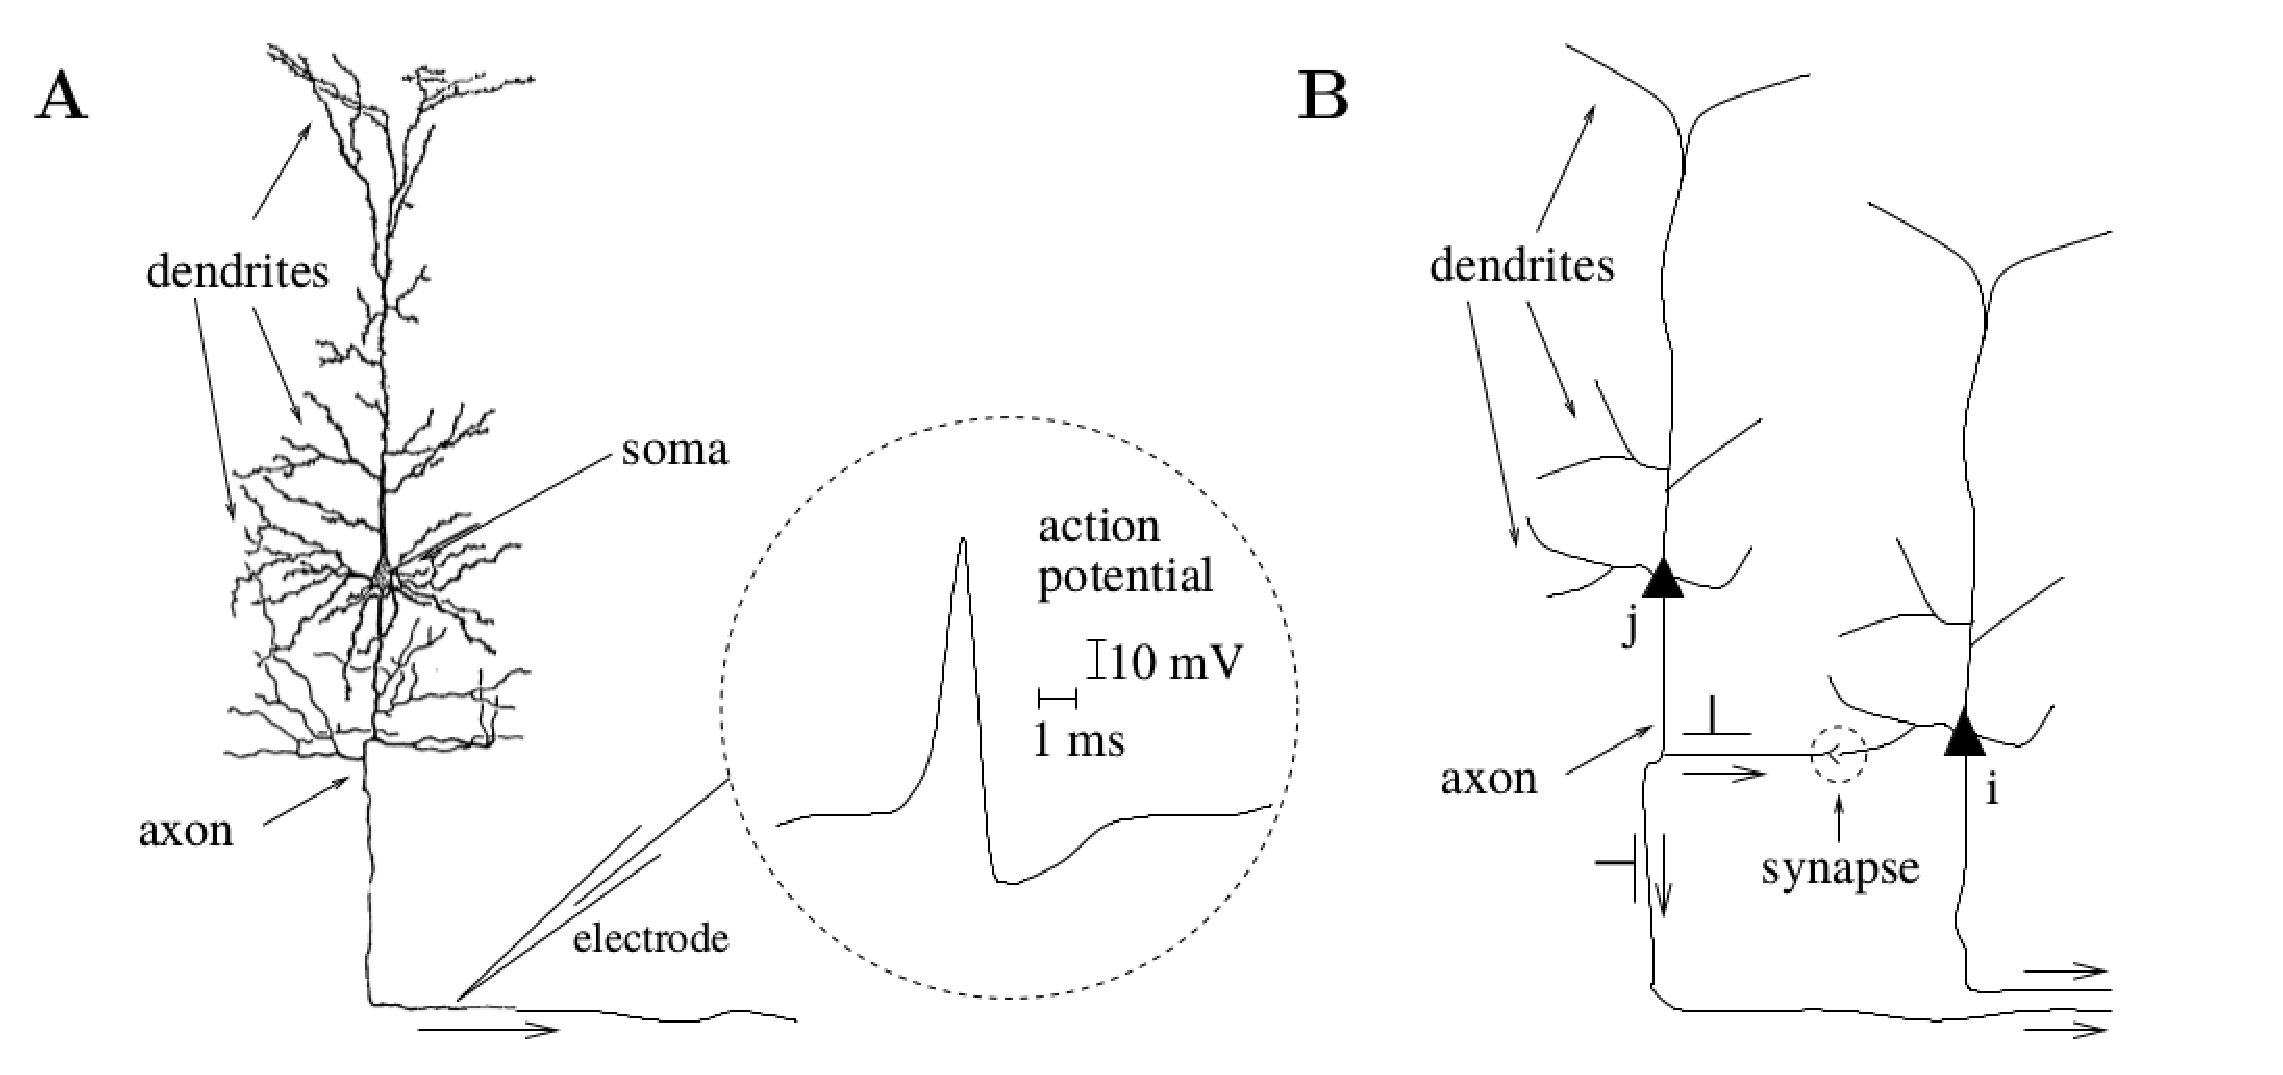
\includegraphics[width=0.85\textwidth]{imgs/Neuron_model.eps}
	\caption{Neuron visualization. Image source \cite{Gerstner2002}}
	\label{fig:biological_neuron}
\end{figure}
Biological neurons exchange information by sending short and sudden pulses, so-called action potentials or spikes.
\todo{include some text here referring to fig \ref{fig:biological_neuron}}
Whenever the membrane potential of a neuron, which can be in- or decreased by incoming spikes depending on the synaptic weight, reaches a certain threshold, the neuron produces a spike itself and resets its membrane potential afterwards \cite{Gerstner2002, Paugam2009}.
Recent neuroscientific research suggests that the exact timing of those spikes encodes information rather than just average firing rates \cite{Bohte2004}.
While traditional \acp{ANN} used in machine learning neglect these biological details, \acp{SNN} embody these spike times and are therefore often referred to as the third generation of neural networks \cite{Maass1997, Paugam2009}.
Maass showed in \cite{Maass1997}, that \acp{SNN} have at least the same computational power as threshold and sigmoidal neural networks of similar size.\\
The simplest spiking neuron model is the \acf{LIF} model with 
\begin{equation}
\frac{\partial V}{\partial t}(t) = - \frac{1}{\tau_{m}} \left( V\left(t\right) - R \cdot I\left(t\right) \right)
\label{eq:LIF}
\end{equation}
\begin{figure}
	\centering
	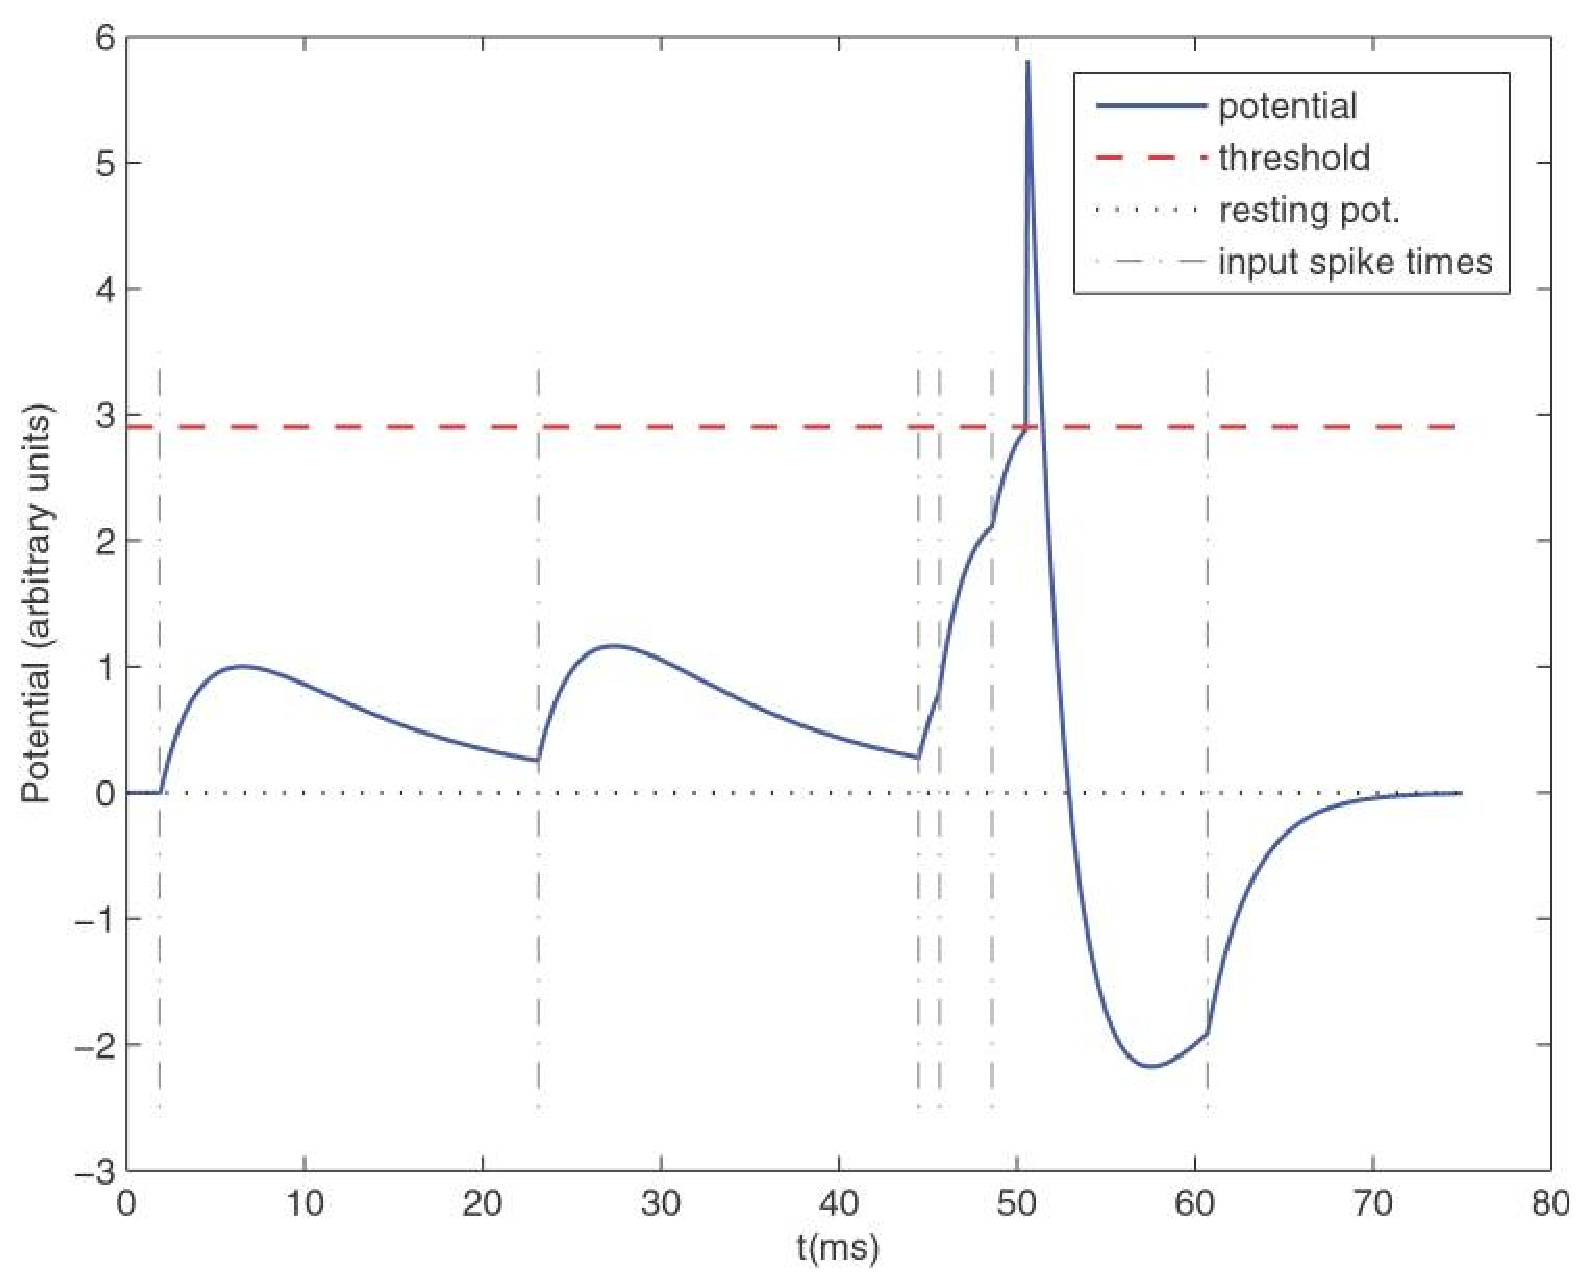
\includegraphics[width=0.75\textwidth]{imgs/LIF_Neuron.eps}
	\caption{Neuron visualization. Image source \cite{Masquelier2007}}
	\label{fig:lif_neuron_model}
\end{figure}
describing the subthreshold behaviour of the neuron, where $V$ is the voltage across the membrane, $I(t)$ is the input current, $R$ is the passive membrane resistance and $\tau_{m}$ is the membrane time constant.
Simply put, equation \ref{eq:LIF} states as follows: the membrane voltage increases in the presence of input current $I(t)$ depending on the membrane resistance $R$ while at the same time, especially in the absence of input current ($I(t)=0$), the voltage decreases or "leaks out" depending on the membrane time constant $\tau_{m}$.
When the voltage $V(t)$ passes a certain threshold $\vartheta$, the neuron produces a spike and the voltage is reset to a resting state $c$ for a certain refractory time interval $\tau_{ref}$ during which incoming spikes have no impact on the membrane potential.
Figure \ref{fig:lif_neuron_model} shows an an example curve of the membrane potential of one \ac{LIF} neuron based on six incoming spikes and visualizes the previously described behaviour. \todo{wording?}
The \ac{LIF} model, despite its biological simplifications, is maybe the most widely used neuron model for simulations due to its simplicity and comparably low computational complexity \cite{Izhikevich2004}, which allows simulations of large networks of neurons in reasonable time.
In contrast, the famous Hodgin-Huxley-model \cite{Hodgkin1952} with its four differential equations and dozens of (biologically meaningful) parameters is the model of high biological plausibility but also computationally challenging regarding large simulations \cite{Izhikevich2004}.
In 2003, Izhikevich proposed a neuron model \cite{Izhikevich2003} as compromise between biological plausibility and computational feasibility.
He showed that this simple model, described by two differential equations with four parameters, is able to produce all known spiking behaviours observed in cortical neurons \cite{Izhikevich2004}. \\
One major hindrance for the widespread adoption of \acp{SNN} has been the problem, that standard learning algorithms for traditional \acp{ANN} like backpropagation \cite{Werbos1974} can not be directly applied to \acp{SNN}.
Although an analogon, the so-called SpikeProp algorithm \cite{Bohte2002} for \acp{SNN} has been developed, the more natural approach is to transfer and mimic biologically inspired learning approaches like Hebbian learning \cite{Hebb1949} or \ac{STDP} \cite{Bi2001}.
An overview of several learning approaches for \acp{SNN} possibly applied with neuromorphic hardware can be found in \cite{Walter2015}.
Another possibility is to train a traditional \ac{ANN} and convert the resulting network into a \ac{SNN} \cite{Diehl2015, Hunsberger2015}.
An example for this approach is the network performing the visual digit recognition task as part of the larger \ac{Spaun} model \cite{Eliasmith2012}, which was derived by training a \ac{DNN} consisting of four \ac{RBM} layers and converting this network using the principles of the \ac{NEF} \cite{Eliasmith2003}.
Although theroretically superior \cite{Maass1997}, \acp{SNN} have not yet outperformed state-of-the-art \acp{DNN} in terms of accuracy in practical machine learning applications \cite{Schmidhuber2015}.\\
Beside the aforementioned procedures to solve traditional machine learning tasks with \acp{SNN} and thereby encode artificial functions in spiking neurons, a different approach is to try to understand how complex cognitive behaviours and the underlying neural functions are performed in the brain.
Therefore, the question how the brain encodes complex information and behaviour in trains of spikes and also how to decode these spike trains to reconstruct the encoded information needs to be answered. 
Although modern research has shed some light on this question regarding the neural code, it is still mainly unanswered as we do not fully understand the anatomical and neurophysiological processes within the brain \cite{Stanley2013}.
Currently, there exist several approaches to code information as spike trains, which can be summarized by the categories rate coding, temporal coding \cite[Chap. 7.6]{Gerstner2014}, population coding \cite[Chap. 1]{Gerstner2002}, \cite{Ponulak2011, Boerlin2011} or sparse coding \cite{Olshausen1996}.
Except for the biologically unrealistic rate coding approach, there are cues for all of these coding schemes and even combinations \cite{Gupta2014} of them to appear in biological systems.


%The term "neuromorphic" was first introduced by Carver Mead in \cite{Mead90}, when describing one of the first silicon retinas.
%For clarity, a first broad definition is provided, which will need some refinement while proceeding in this section:
%\begin{defn}
%\label{def:neuromorph}
%Artificial systems, that share organization principles with biological nervous systems are called \textbf{neuromorphic}.
%\end{defn} 
%Biologically inspired systems and algorithms have seen significant progress and achieved remarkable results, e.g. in the field of machine learning, despite some simplifications in terms of biological accuracy.
%So-called first and second generation \ac{ANN} described in \ref{subsec:ML_ANN} are also covered by definition \ref{def:neuromorph} as neuromorphic systems, although they neglect some biological details.
%\subsection{Spiking Neural Networks}
%Biological neurons exchange information by sending short and sudden increases in their membrane voltage, so-called action potentials or spikes.
%Recent neurological research suggests that the exact timing of those spikes encodes information rather than just average firing rates (\todo{Citation}).
%While \ac{ANN} of the first two generations neglect these biological details, recent neural networks structures, so-called \ac{SNN} \cite{Paugam2009}, embody these spike times and are therefor often referred to as the third generation of neural networks . 
%
%
%
%\label{subsec:spiking_neural_nets}
%
%\subsection{Neural Modelling}
%\subsection{Neuromorphic Hardware}
%The field of neuromorphic computing achieved several significant advances in recent years, massively increasing the number of neurons simultaneously available in complex models and achieving real-time (less than $\SI{100}{\milli\second}$) execution through hardware implementation. 
%This basic research is resulting in semiconductor implementations becoming available on a wider scale, such as University of Manchester's \ac{SpiNNaker} Chip \cite{Furber2014} or IBM’s recently announced True North \cite{Akopyan2015} architecture.
%\section{Traditional Computing}